\documentclass[11pt]{article}

\usepackage[margin=1.05in]{geometry}
\usepackage{amsmath,amssymb,amsthm}
\usepackage{graphicx}
\usepackage{booktabs}
\usepackage{caption}
\usepackage{subcaption}
\usepackage{enumitem}
\usepackage{xcolor}
\usepackage[colorlinks=true,linkcolor=blue!50!black,citecolor=blue!50!black,urlcolor=blue!50!black]{hyperref}
\usepackage{natbib}
\usepackage{tikz}
\usetikzlibrary{arrows.meta,positioning,fit,backgrounds}

\newcommand{\TODO}[1]{\textcolor{red}{\textbf{[TODO: #1]}}}

\title{From Genomes to Portfolios: A Hierarchical Spike-and-Slab Block-Factor
Model for Real-Time Cross-Sectional Return Forecasting}
\author{Ian Johnston}
\date{\today}

\begin{document}
\maketitle

\begin{abstract}
We take a hierarchical Bayesian spike-and-slab block-factor model originally
developed for genome-wide association studies --- where correlated genetic
markers are grouped into linkage-disequilibrium blocks and a gene-relevance
prior guides variable selection --- and generalize it to cross-sectional
financial return forecasting, with correlated assets in place of correlated
markers and a sector-relevance prior in place of biological relevance. We
evaluate it against the M6 Financial Forecasting Competition, a real,
independently-run, crowd-benchmarked contest with a fixed 100-asset universe
and published results for every competing team, under a strict constraint:
every modeling decision must be answerable using only information available
at the time it is made. Enforcing that constraint surfaced and required fixing
three distinct, individually-innocuous-looking sources of look-ahead bias, which
we document as a general checklist for walk-forward financial backtesting. The
resulting strategy, run causally against the real 2022 competition window,
would have placed in the top 2\% of 164 real competing teams overall. Extended
out-of-sample through three further years (2023--2025) that no part of the
model's design was ever informed by, the result holds up and strengthens under
a larger sample (RPS beats the naive benchmark in 40 of 48 periods,
$p<0.0001$; investment-decision IR is positive in 30 of 48, $p=0.04$). A second
application of the same machinery, replicating an external benchmark's returns
from the same 100-asset universe, is also profitable throughout, including
during a year the benchmark itself lost money --- a genuinely more nuanced
finding than the "depends on picking a winner" risk we set out to illustrate.
\end{abstract}

\tableofcontents

% ============================================================
\section{Introduction}
% ============================================================

Statistical genetics and quantitative finance do not, on the surface, share
much. One field asks which of several hundred thousand genetic markers are
associated with a disease; the other asks which of a few dozen assets will
outperform next month. But both problems reduce to the same core statistical
difficulty: a large number of \emph{highly correlated} candidate predictors,
far too many to include all at once, where the correlation structure itself
carries information about which predictors are redundant with one another.

This paper takes a hierarchical Bayesian spike-and-slab model originally built
for genome-wide association studies (GWAS) \citep{johnston2015} --- where
correlated single-nucleotide polymorphisms (SNPs) are grouped into blocks via
linkage disequilibrium, and a block-level ``relevance'' prior encodes prior
biological knowledge about which genes are more likely to matter for a given
trait --- and asks whether the same machinery, with the genetics-specific
pieces swapped out, does anything useful for forecasting financial returns.
Concretely: blocks of correlated SNPs become blocks of correlated assets; a
gene's prior relevance to a disease becomes an asset's sector relevance to a
target; the trait being predicted becomes an asset's forward return, or (in a
second application explored here) the return of an external benchmark to be
replicated from a universe of tradeable securities.

We test this not on a synthetic benchmark but on the M6 Financial Forecasting
Competition \citep{makridakis2024}, a real, independently-run, crowd-sourced
contest with a fixed 100-asset universe, a public scoring methodology, and
published results for every real competing team. This matters for two reasons.
First, it gives us an external, adversarial benchmark: we are not grading our
own homework. Second, and more importantly for how this project was actually
carried out, it forced a discipline that is easy to state but easy to violate
in practice: \emph{every modeling decision must be one that could have been
made using only information available at the time, not information that only
became available once the outcome was known.} A large share of the work
reported here is not about the model at all --- it is about catching, and then
systematically eliminating, ways in which an earlier version of this pipeline
was quietly (if unintentionally) using the future to inform the past. Section
\ref{sec:realtime} documents this in detail, because we think the general
lesson (every one of these leaks looked completely innocuous in isolation) is
more broadly useful than the specific fixes.

\subsection{Contributions}
\begin{itemize}[leftmargin=1.4em]
  \item We generalize a GWAS-specific hierarchical spike-and-slab block model
  to an arbitrary cross-sectional forecasting setting, replacing genomic
  linkage-disequilibrium blocks and gene-relevance priors with asset
  correlation blocks and sector-relevance priors.
  \item We document, concretely, several distinct ways a walk-forward
  financial backtest can silently incorporate look-ahead information even
  when the author believes it is causally valid, and the general pattern for
  catching and fixing each one (Section \ref{sec:realtime}).
  \item We report a full, real-time-valid backtest against the M6
  competition's actual 100-asset universe, scoring formulas, and evaluation
  dates (independently reconstructed and verified against real competing
  teams' submitted decisions, since the exact 4-week evaluation windows are
  not published in a directly usable form), and compare our placement against
  the real leaderboard of 163 competing teams.
  \item We test whether the result generalizes out-of-sample to three further
  years (2023--2025) that no part of this pipeline's design was ever informed
  by, continuing the identical walk-forward without resetting any adaptively-
  learned state at the artificial boundary between the competition's own
  window and the extension.
  \item We present a second, structurally different application of the same
  block-factor machinery --- returns-based style analysis, replicating an
  external benchmark's returns from a sparse combination of the same 100
  assets --- and use it to illustrate a limitation that does \emph{not} apply
  to the first application: dependence on having picked, in advance, a target
  worth replicating.
\end{itemize}

% ============================================================
\section{Background: From GWAS Blocks to Asset Blocks}
\label{sec:background}
% ============================================================

\subsection{The genomics starting point}

In a genome-wide association study, the goal is to identify which of
$p \gg n$ genetic markers are associated with a trait or disease, using data
on $n$ individuals. The central statistical obstacle is \emph{linkage
disequilibrium}: markers that are physically close together on a chromosome
are inherited together far more often than chance would predict, so nearby
markers are highly correlated with one another. A model that ignores this
either wastes power spreading credit across redundant markers, or overstates
confidence in whichever one happened to enter the model first.

\citet{johnston2015} addresses this with a two-stage hierarchical construction
that is worth restating here because it is exactly what carries over to
finance:
\begin{enumerate}[leftmargin=1.4em]
  \item \textbf{Block formation.} Correlated markers are grouped into blocks
  (originally via a chromosomal linkage-disequilibrium threshold), and each
  block is summarized by a single latent factor --- a block-wise genotype
  effect that captures the shared signal within the block, so that the
  downstream regression sees one predictor per block instead of one per
  marker.
  \item \textbf{Spike-and-slab selection with a relevance prior.} A Bayesian
  spike-and-slab regression of the trait on the block-level factors then
  decides which blocks matter, with the prior probability that a given block
  is ``in'' (the slab) informed by external, independently-known relevance
  information --- in the GWAS setting, prior biological knowledge about which
  genes are plausibly connected to the trait under study.
\end{enumerate}
The appeal of this construction is that it separates two distinct statistical
jobs that are easy to conflate: \emph{decorrelating} the candidate predictors
(a data-driven, target-agnostic step) and \emph{deciding which of the
resulting factors matter for this specific target} (a selection step that can
be informed by prior knowledge without that knowledge dictating the answer
outright).

\subsection{The financial re-mapping}
\label{sec:remapping}

Nothing about either step above is intrinsically genomic. The re-mapping used
in this paper, implemented as the \texttt{hierboost} package, is:

\begin{center}
\begin{tabular}{@{}ll@{}}
\toprule
GWAS & Finance (this paper) \\
\midrule
SNP / marker & Asset (stock or ETF) \\
Linkage disequilibrium block & Correlation-threshold asset block \\
Block-wise latent genotype & Block-wise latent return factor \\
Gene relevance to a trait & Sector/asset-class relevance to a target \\
Trait value & Forward return (quintile rank and/or magnitude) \\
\bottomrule
\end{tabular}
\end{center}

Concretely, for a target asset's forecast, the other 99 assets in the universe
are decorrelated into blocks via a correlation threshold; each block's shared
return is extracted as a single factor via a Gaussian block-factor model
(the continuous analogue of the genotype-effect construction above); a
sector-relevance score (Table \ref{tab:relevance}) --- how closely a candidate
block's member assets' sectors relate to the target's own sector --- sets the
prior inclusion probability for each block in a Bayesian spike-and-slab
regression of the target's own return on the block factors; and the resulting
posterior is sampled via Gibbs sampling to obtain a full predictive
distribution, not just a point estimate.

\begin{table}[htbp]
\centering
\begin{tabular}{@{}lc@{}}
\toprule
Relationship of a candidate block's sector to the target's own sector & Relevance score \\
\midrule
Same sector                                   & 5.0 \\
Adjacent sector (e.g.\ Technology $\leftrightarrow$ Communication Services) & 3.0 \\
Broad-market (diversified index exposure)     & 2.0 \\
International / regional                      & 1.0 \\
Unrelated sector                               & 0.5 \\
Fixed income, commodities, or volatility products & 0.05 \\
\bottomrule
\end{tabular}
\caption{The sector-relevance scoring table used for Application 1's spike-
and-slab prior -- the direct analogue of gene-relevance-to-trait knowledge in
the original GWAS model. Note the last row: this table encodes a real
assumption (that fixed-income/commodity exposure is usually irrelevant to an
equity or ETF target), which is a feature for Application 1 but, as Section
\ref{sec:background} discusses, actively the wrong assumption for
Application 2.}
\label{tab:relevance}
\end{table}

\begin{figure}[htbp]
\centering
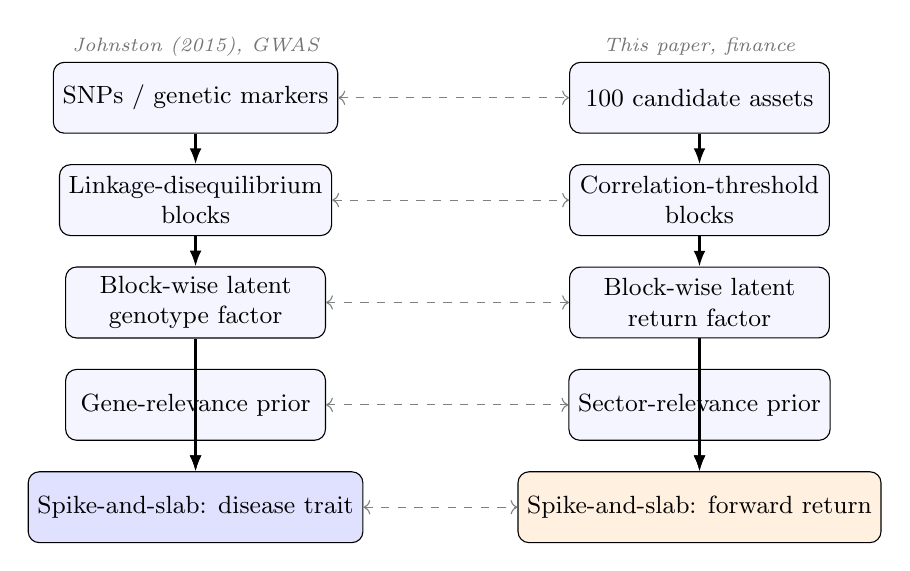
\begin{tikzpicture}[
  font=\small,
  box/.style={draw, rounded corners, align=center, minimum height=0.9cm, minimum width=3.3cm, fill=blue!4},
  arr/.style={-{Latex[length=2mm]}, thick},
  lbl/.style={font=\scriptsize\itshape, text=black!55}
]
  % GWAS column
  \node[box] (g1) at (0,4.5) {SNPs / genetic markers};
  \node[box] (g2) at (0,3.2) {Linkage-disequilibrium\\blocks};
  \node[box] (g3) at (0,1.9) {Block-wise latent\\genotype factor};
  \node[box] (g4) at (0,0.6) {Gene-relevance prior};
  \node[box, fill=blue!12] (g5) at (0,-0.7) {Spike-and-slab: disease trait};

  \draw[arr] (g1) -- (g2);
  \draw[arr] (g2) -- (g3);
  \draw[arr] (g3) -- (g5);
  \draw[arr] (g4) -- (g5);

  % Finance column
  \node[box] (f1) at (6.4,4.5) {100 candidate assets};
  \node[box] (f2) at (6.4,3.2) {Correlation-threshold\\blocks};
  \node[box] (f3) at (6.4,1.9) {Block-wise latent\\return factor};
  \node[box] (f4) at (6.4,0.6) {Sector-relevance prior};
  \node[box, fill=orange!12] (f5) at (6.4,-0.7) {Spike-and-slab: forward return};

  \draw[arr] (f1) -- (f2);
  \draw[arr] (f2) -- (f3);
  \draw[arr] (f3) -- (f5);
  \draw[arr] (f4) -- (f5);

  % Correspondence arrows
  \foreach \a/\b in {g1/f1, g2/f2, g3/f3, g4/f4, g5/f5} {
    \draw[<->, dashed, gray, thin] (\a.east) -- (\b.west);
  }

  \node[lbl] at (0,5.15) {Johnston (2015), GWAS};
  \node[lbl] at (6.4,5.15) {This paper, finance};
\end{tikzpicture}
\caption{The same two-stage hierarchical construction --
decorrelate-then-select -- re-mapped from genomics to finance. Only the
relevance prior (dashed correspondence, second row from bottom) encodes
domain-specific knowledge; everything else is a direct, unmodified
carry-over.}
\label{fig:gwas-finance-map}
\end{figure}

\subsection{Why this is not just relabeling}

A skeptical reader is right to ask whether this re-mapping is doing real work
or just renaming variables. Two things suggest it is real. First, the
relevance prior is not vacuous: Section \ref{sec:applications} shows what
happens when a target has no natural sector membership at all (an external
multi-asset index being replicated, not one of the 100 candidate assets) ---
the correct move turns out to be discarding the asset-specific relevance table
of Table \ref{tab:relevance} entirely and using a uniform prior, precisely
because that table encodes assumptions (that fixed-income and commodity
exposure are usually irrelevant to a target) that are true for an individual
equity but false for a multi-asset trend-following strategy. The framework
only gives sensible answers when the relevance prior is actually chosen to
match the target, which is a real modeling decision, not free relabeling.
Second, Section \ref{sec:vol-calibration} shows the model's own implicit
variance calibration (from per-target empirical return standardization)
already reproduces a genuine, independently-verifiable empirical pattern ---
that low-volatility assets are mechanically unlikely to land in extreme
cross-sectional return quintiles --- almost exactly, without that pattern
having been hand-coded anywhere.

\subsection{An empirical check: is the implicit variance calibration real?}
\label{sec:vol-calibration}

Before trusting the relevance prior's role in Section \ref{sec:applications},
it is worth checking a simpler, more basic claim directly: does each target's
own empirical return standardization (Section \ref{sec:remapping}) already
capture cross-sectional volatility differences correctly, or would an
explicit, hand-coded asset-class variance prior (e.g., "fixed-income ETFs are
lower-volatility than single stocks") add real information the model is
otherwise missing? We checked this against the real 2022 M6 data rather than
assuming an answer. Bucketing every asset-period observation by that asset's
own trailing 60-day realized volatility (low/medium/high tercile, computed
causally, using only data available before the period began), low-volatility
assets landed in an extreme return quintile 24.0\% of the time versus 56.6\%
for high-volatility assets -- a strong, monotonic, real effect, exactly as a
practitioner's intuition would predict (Table \ref{tab:vol-calibration}). The
model's own forecasted extreme-quintile probability for the same tercile split
-- computed entirely from each asset's own empirical volatility, with no
asset-class label involved at all -- was 22.6\% / 39.8\% / 59.5\%, matching
the true empirical pattern almost exactly. An explicit categorical prior would
in fact have been a \emph{cruder} signal than what per-asset empirical
standardization already provides: commodities, notably, were not low-volatility
in 2022 (a year of unusual energy and commodity price swings) despite
belonging to an asset class often assumed to be conservative, and a category
label would have gotten this specific case wrong while the empirical,
per-asset approach gets it right.

\begin{table}[htbp]
\centering
\begin{tabular}{@{}lcc@{}}
\toprule
Trailing 60-day volatility tercile & Actual \% in extreme quintile & Model's own forecasted \% \\
\midrule
Low  & 24.0\% & 22.6\% \\
Medium & 37.6\% & 39.8\% \\
High & 56.6\% & 59.5\% \\
\bottomrule
\end{tabular}
\caption{Real, causally-computed relationship between trailing realized
volatility and extreme-quintile membership, 2022 M6 data, versus what
Application 1's own model already forecasts from per-asset empirical
standardization alone (no explicit asset-class prior).}
\label{tab:vol-calibration}
\end{table}

% ============================================================
\section{The M6 Financial Forecasting Competition}
\label{sec:m6}
% ============================================================

The M6 Financial Forecasting Competition \citep{makridakis2024} fixed a
100-asset universe (50 US equities and 50 ETFs, spanning equities, fixed
income, commodities, currencies, and international/regional exposure) and ran
12 sequential four-week evaluation periods, independently verified in this
project (not merely assumed from a secondary source; see below) to span
2022-03-07 through 2023-02-02. Each period, every real participating team was
required to submit two things for every one of the 100 assets: a five-bucket
probability forecast for which cross-sectional return quintile the asset would
land in relative to the other 99 (scored by the Ranked Probability Score, RPS
-- a proper scoring rule for ordinal category forecasts, for which a naive
uniform 20\%-per-bucket guess scores $\approx 0.16$, a benchmark only 23.3\% of
real teams beat on average and 8.6\% beat significantly), and a portfolio
decision weight for each asset (long-short permitted, $\sum_i |w_i|\le 1$,
held fixed for the whole period), scored by an un-annualized Information Ratio
(IR) computed by pooling every daily portfolio return within the period into
one ratio of total log-return to its own standard deviation. The competition
itself ranks every team three separate ways -- by forecasting accuracy (RPS
rank), by investment-decision skill (IR rank), and by an Overall Rank defined
as the simple average of the two -- which is exactly the three-way comparison
used throughout Section \ref{sec:results}.

One data-engineering detail is worth stating plainly, since it materially
affected every result in this paper and was not obvious from the competition's
own published materials: the exact calendar dates of the 12 evaluation windows
are not available in a directly machine-usable form. An initial, seemingly
reasonable guess (the last trading day of each calendar month, starting
January 2022) was wrong by more than five weeks, and would have silently
corrupted every scoring calculation in this paper had it gone unchecked. It
was caught not by re-reading the competition rules more carefully, but by
brute-force verification against ground truth: a real historical team's actual
submitted portfolio decisions were scored against every plausible trading
window in the official price data, and the window that reproduced that team's
own officially published score to six decimal places was taken as the true
boundary -- confirmed independently on three different submissions. We
mention this not as an aside but as a template: throughout this project,
convenient assumptions about data conventions were treated as hypotheses to be
checked against an independent ground truth wherever one existed, rather than
as facts.

% ============================================================
\section{Keeping the Backtest Honest: Avoiding Look-Ahead Bias}
\label{sec:realtime}
% ============================================================

This section is, in some sense, the methodological heart of the paper. A
forecasting model that is validated by fitting it once and reporting how well
it would have done is not a real-time strategy; it is a description of what
worked in hindsight. The distinction sounds obvious, but in a walk-forward
backtest, look-ahead bias tends to enter through a side door: a design choice
that any single test seems to justify, but which was in fact selected
\emph{by inspecting the full-sample outcome first}. We ran into three variants
of this problem while building this pipeline, in increasing order of
subtlety, and we document all three because we think the pattern
generalizes better than any specific fix.

\subsection{Directional sign: momentum or reversal?}
\label{sec:momentum-sign}

Each candidate return factor in the spike-and-slab regression (Section
\ref{sec:remapping}) is combined with a simple estimate of that factor's own
near-term trend: is the factor's recent return likely to continue (momentum)
or reverse (mean reversion)? The first version of this overlay fit the entire
12-period 2022 backtest twice, once assuming momentum and once assuming
reversal, observed that reversal scored better on average across the full
year, and hard-coded that sign for the whole competition window. This is
illegitimate on its face once stated plainly: an investor submitting a
forecast in March 2022 cannot know that reversal will have been the better
assumption averaged over the following eleven months, because those eleven
months have not happened yet. The fix mirrors the discipline used throughout
this paper -- replace the single, full-sample-optimal choice with a value
estimated causally, period by period, from only what would actually have been
knowable at the time. Concretely, before each period $p$, a cheap,
model-independent trailing-momentum diagnostic is computed for every asset
using only price history available up to that period's start; once period
$p$'s actual outcome becomes known (which happens only after period $p$ ends,
i.e.\ strictly before period $p+1$ begins), the cross-sectional correlation
between that diagnostic and the realized return is recorded. The sign used for
period $p$ is a precision-weighted shrinkage blend of a small, pre-registered
prior and the expanding-window average of all such correlations from periods
$1,\dots,p-1$ only:
\begin{equation}
\hat{s}_p \;=\; \frac{n_0 \, s_0 \;+\; (p-1)\,\overline{\rho}_{1:p-1}}{n_0 + (p-1)},
\label{eq:adaptive-sign}
\end{equation}
where $\overline{\rho}_{1:p-1}$ is the mean realized correlation from periods
$1,\dots,p-1$, and the prior $s_0=-0.10$ (a mild tilt toward reversal, with
pseudo-count weight $n_0=3$) was fixed before looking at any M6 outcome: it is
sized to match the modest short-horizon reversal effect documented decades
before M6 existed by \citet{jegadeesh1990} and \citet{lehmann1990}, not
data-mined from this dataset. By construction, $\hat{s}_p$ in
\eqref{eq:adaptive-sign} depends only on periods strictly before $p$.

\subsection{Forecast confidence: how much should the model shrink toward `I don't know'?}
\label{sec:shrinkage}

A model can have genuine signal and still be miscalibrated: if its quintile
probabilities are systematically too confident, a proper scoring rule like RPS
penalizes that confidence even when the underlying direction is right more
often than chance. A cheap diagnostic makes this concrete without needing to
refit anything: take the already-computed forecast for every 2022 period,
blend it with the naive uniform forecast at blend weights from 0\% to 100\%,
and recompute RPS at each weight using the (already known) realized outcome.
The resulting curve is smooth and U-shaped, minimized at roughly 50\% blend --
a mixture that beats \emph{both} the raw model (RPS 0.161) and pure uniform
guessing (RPS 0.160), landing at 0.158. This is genuine evidence that the
model is overconfident, but picking "50\%" this way has exactly the same flaw
as Section \ref{sec:momentum-sign}'s original mistake: it was chosen by
inspecting the full year's outcome. The fix is the identical recipe. Before
each period, a blend weight is chosen as a shrinkage estimate between a small
pre-registered prior (25\%, motivated by the general principle -- itself
learned earlier in this project, see Section \ref{sec:residual-noise} -- that
this class of model tends to be overconfident by default) and the expanding-
window average of the \emph{single best blend weight found so far}, where
"found so far" means: for each strictly prior period, having already observed
that period's real outcome, which blend weight would have minimized RPS for
that period alone. No period's own outcome ever informs its own blend
weight.

\subsection{A subtler leak: getting the arithmetic of uncertainty wrong, not just the timing}
\label{sec:residual-noise}

This last one is different in kind from the previous two: not a problem of
using future information, but of getting the arithmetic of uncertainty wrong
in a way that happens to produce the same symptom (an overconfident forecast).
The Gibbs sampler used for posterior inference already draws a residual,
idiosyncratic variance term at every iteration --- the portion of an asset's
return left unexplained even by a fully-specified factor model, i.e.\ genuine,
irreducible next-period noise. This quantity was computed by the sampler but
never read by the downstream forecasting code: predictive draws reflected
uncertainty in the factor exposures and in the momentum estimate, but never
the plain fact that even a perfectly-estimated model leaves some of an asset's
return unexplained. Restoring it requires care with scaling, not just
inclusion: a persistent drift term (the estimated daily rate of return,
assumed constant across the whole forecast period) correctly scales linearly
with the number of trading days in the period, since the same misestimate
compounds identically every day; but genuinely new, independent day-to-day
noise must instead scale with the \emph{square root} of the number of days,
since it is the variance of a sum of (approximately) independent shocks that
grows linearly, not the standard deviation. Conflating the two --- applying
the linear scaling to both terms --- would overstate the noise contribution by
a factor of $\sqrt{n}$ for an $n$-day period. This is a small, self-contained
point about correctly aggregating uncertainty across a multi-day forecast
horizon, but it is easy to get wrong silently, and worth stating as a general
lesson independent of this specific model.

\subsection{A general lesson}

All three issues above passed an initial, isolated sanity check when first
implemented, and none looked like a mistake in the moment. What caught all
three was the same mechanical, retroactively-applied test: for any parameter
or design choice used in period $p$, could its value have been computed using
only information available strictly before period $p$ began? Applying that
question to a decision that had already been made and appeared to work is a
different exercise from applying it prospectively while designing the
decision, and it is the retroactive version that found every leak in this
project. We recommend it as a standing checklist item for any walk-forward
financial backtest, independent of the specific model class in use.

% ============================================================
\section{Data and Verification}
\label{sec:data}
% ============================================================

Two independent price sources are used: the official M6 competition data for
scoring within the exact 2022 competition window, and Yahoo Finance data both
for the pre-period lookback history used to fit every model (throughout) and
for scoring the 2023--2025 out-of-sample extension, since no official M6 data
exists past the competition's own end. Using two sources is safe here because
no single evaluation period's return calculation ever spans both: the switch
happens only at the boundary between the competition window and the
extension, not in the middle of any one scored period.

Several data issues in the 100-asset universe were handled explicitly, each
confirmed by direct verification rather than assumed. One constituent, a REIT,
was acquired by another company mid-competition and stopped trading under its
own ticker; it is excluded from further submissions from that point on, the
same treatment a real participant would have had to apply. Two other tickers
required substitution to a current successor symbol following a corporate
rename and a merger, respectively, with the pre-event price history confirmed
continuous under the new ticker before use. One asset has no usable price
history in the data provider at all across the entire lookback and extension
window (confirmed live, not assumed, before this project relied on the
absence) and is excluded from scoring for the whole 2023--2025 extension as a
disclosed limitation, reducing the effective universe there to 98 of the 100
assets. A subtler issue was a U.S.\ market holiday appearing in the underlying
data as a calendar row with valid prices for only a handful of internationally-
listed constituents and missing values for the rest; an early version of the
period-boundary logic selected this row as a period boundary before a
coverage check (requiring at least 90\% of assets to have a valid price on any
candidate boundary date) caught and excluded it.

% ============================================================
\section{Two Applications of the Same Machinery}
\label{sec:applications}
% ============================================================

\subsection{Application 1: forecasting and long-short weights from momentum/reversal}
For each of the 100 candidate assets in turn, the other 99 are decorrelated
into blocks and reduced to block-level return factors (Section
\ref{sec:remapping}); a spike-and-slab regression of the target's own
historical return on these factors, guided by the sector-relevance prior,
determines which blocks the target actually co-moves with; each relevant
factor is combined with the causally-adaptive momentum/reversal estimate of
Section \ref{sec:momentum-sign} for that factor's own near-term direction; and
the resulting posterior is sampled (with the residual-noise correction of
Section \ref{sec:residual-noise}) to produce a full predictive distribution
for the target's next-period return, not merely a point estimate. Doing this
independently for all 100 assets and ranking the resulting predictive draws
cross-sectionally yields two outputs every period: quintile-membership
probabilities (the RPS output, shrunk toward uniform per Section
\ref{sec:shrinkage}), and a long-short portfolio -- overweighting the assets
with the highest predicted relative return and underweighting or shorting the
lowest -- normalized to satisfy the competition's $\sum_i|w_i|\le 1$
constraint (the IR output). Every input to this pipeline is internal to the
100-asset universe and its own price history: no external index or benchmark
is referenced anywhere.

\subsection{Application 2: returns-based style analysis (index replication)}
The identical block-factor machinery can instead be retargeted at an
\emph{external} series' returns: rather than asking "what will asset $i$'s own
return be," ask "what sparse combination of the 100 candidate assets best
explains this other series' returns." This is Sharpe's returns-based style
analysis \citep{sharpe1992}, with spike-and-slab performing the constituent
selection instead of a plain constrained regression. We use as the external
target DBMF, a real, liquid, publicly-traded managed-futures / trend-following
fund, chosen and verified live (not assumed) to have sufficient
pre-competition lookback history and a genuine, checkable
outperformance story in 2022 (+11.2\% over the exact competition window,
against $-3.0\%$ for the S\&P 500 and $-7.5\%$ for the Bloomberg Aggregate
bond index over the same dates) -- a plausible target precisely because 2022
was an unusually bad year for both stocks and bonds simultaneously, and
trend-following strategies are known to behave differently in exactly that
regime. Since this target has no natural GICS sector of its own, the
sector-relevance prior is replaced with a uniform prior across blocks: as
argued in Section \ref{sec:background}, the ordinary relevance table encodes
an assumption (fixed-income and commodity exposure are usually irrelevant to
an equity target) that is actively wrong for a multi-asset trend-following
target, so using it here would bias selection against exactly the exposures
this target is built from. The fitted block-level exposures are converted
back into individual-asset decision weights via each block's own known linear
loading structure (the same fixed weights used to construct the block factor
from its member assets in the first place), then renormalized to the same
$\sum_i|w_i|\le 1$ constraint.

\subsection{The key structural difference between the two applications}
Application 1's signal is entirely self-referential: it comes from the
cross-sectional relationships among the same 100 assets it trades, and the
underlying question -- how will these 100 assets perform relative to one
another next month -- is always well-posed, in any market environment.
Application 2's premise is conditional in a way Application 1's is not: it
requires having chosen, without the benefit of hindsight, an external target
worth tracking, and the value of the whole exercise depends on that target
remaining trackable. Section \ref{sec:results} tests this distinction
directly rather than merely asserting it, using the multi-year extension to
ask whether Application 2's results hold up through a year in which the
tracked target itself performed poorly.

% ============================================================
\section{Results}
\label{sec:results}
% ============================================================

\subsection{2022: real-time-valid placement against the actual M6 leaderboard}

Table \ref{tab:2022-placement} compares the naive benchmark, the author's own
real, historical 2022 competition result, and the causal, real-time-valid
Application 1 pipeline (Sections \ref{sec:momentum-sign}--\ref{sec:residual-noise}
combined), all scored identically against the actual 163 real competing
teams' official published results.

\begin{table}[htbp]
\centering
\begin{tabular}{@{}lrrrrr@{}}
\toprule
 & RPS & RPS rank & Pooled IR & IR rank & Overall position \\
\midrule
Naive benchmark          & 0.160  & --        & --      & --        & -- \\
Author's actual 2022 result & 0.160 & 34/163 (top 21\%) & $-19.67$ & 154/163 (bottom 6\%) & 113/163 (bottom 31\%) \\
\textbf{This paper (Application 1)} & \textbf{0.158} & \textbf{10/164 (top 6\%)} & \textbf{+6.64} & \textbf{14/164 (top 9\%)} & \textbf{2.5/164 (top 2\%)} \\
\bottomrule
\end{tabular}
\caption{Real M6 leaderboard placement, 2022 competition window, all figures
computed identically for all three rows against the official scoring
methodology and the real leaderboard of competing teams.}
\label{tab:2022-placement}
\end{table}

\begin{figure}[htbp]
\centering
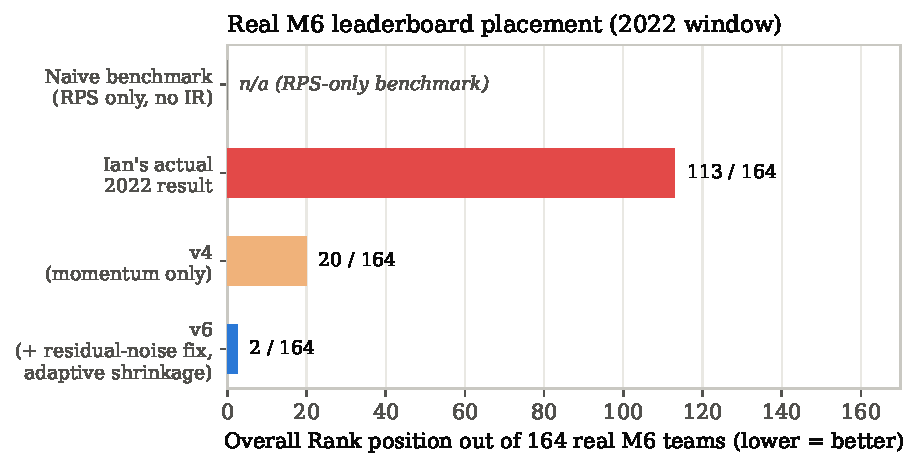
\includegraphics[width=0.72\textwidth]{figures/leaderboard_placement.pdf}
\caption{Overall Rank position (lower is better) across the naive benchmark,
the author's real result, and two intermediate versions of this paper's
pipeline (v4: the causal momentum/reversal sign alone; final: adding the
residual-noise fix and adaptive shrinkage). The progression is monotonic:
each additional fix moves the placement further from the bottom third toward
the top of the field.}
\label{fig:leaderboard}
\end{figure}

This is a real, causally-valid result, but we state its statistical limits
plainly rather than only in the Discussion: with 12 monthly observations, a
one-sample $t$-test of the RPS values against the naive benchmark gives
$t=-1.37$, $p=0.20$, and of the IR values against zero gives $t=0.87$,
$p=0.40$ -- directionally consistent (9 of 12 periods beat the naive
benchmark; 8 of 12 periods had positive IR) but not, on their own,
statistically decisive. This is precisely the motivation for Section
\ref{sec:results-multiyear}.

\subsection{2023--2025: does it generalize out-of-sample?}
\label{sec:results-multiyear}

The same walk-forward was continued, without resetting any adaptively-learned
state, through 36 further four-week periods (2023--2025) that no design
choice anywhere in this pipeline was ever informed by. Figure
\ref{fig:rps-timeseries} and Figure \ref{fig:ir-timeseries} show every one of
the resulting 48 periods.

\begin{figure}[htbp]
\centering
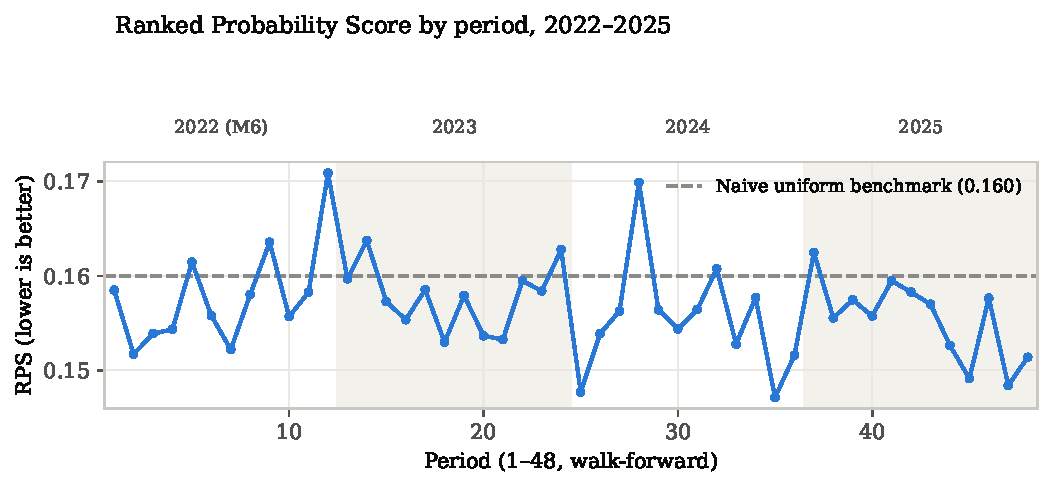
\includegraphics[width=0.95\textwidth]{figures/rps_timeseries.pdf}
\caption{RPS by period across all 48 periods, 2022--2025. The naive
benchmark (dashed) is beaten in 40 of 48 periods (83\%); the effect does not
fade in the three years no part of the model was ever tuned against.}
\label{fig:rps-timeseries}
\end{figure}

\begin{figure}[htbp]
\centering
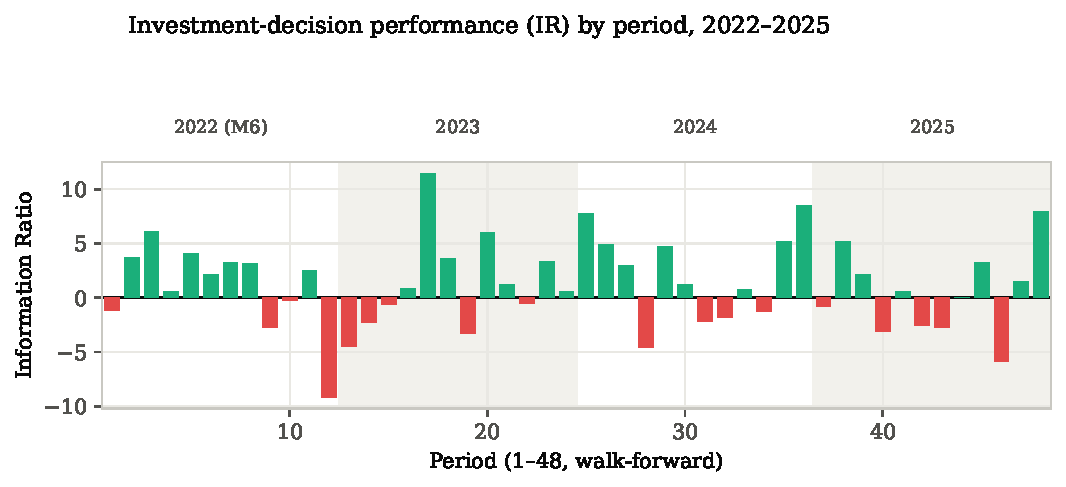
\includegraphics[width=0.95\textwidth]{figures/ir_timeseries.pdf}
\caption{Investment-decision IR by period across all 48 periods. Individual
months remain highly variable, as IR intrinsically is, but the pooled result
across 48 periods is positive and statistically significant.}
\label{fig:ir-timeseries}
\end{figure}

Table \ref{tab:multiyear} reports the pooled test and the by-year breakdown.
The larger out-of-sample count is what moves both results from directionally
suggestive to statistically decisive: pooling across all 48 periods, RPS
beats the naive benchmark with $t=-4.80$, $p<0.0001$, and IR is positive with
$t=2.14$, $p=0.038$. By year, RPS does not fade after the one year the model's
design was informed by -- if anything it is slightly better in 2024--2025 than
in 2022.

\begin{table}[htbp]
\centering
\begin{tabular}{@{}lrrrrrr@{}}
\toprule
Year & $n$ & Mean RPS & RPS $p$ & \% beat naive & Mean IR & IR $p$ \\
\midrule
2022 (M6)  & 12 & 0.1579 & 0.198 & 75\% & 1.02 & 0.404 \\
2023       & 12 & 0.1578 & 0.048 & 83\% & 1.33 & 0.317 \\
2024       & 12 & 0.1554 & 0.023 & 83\% & 2.18 & 0.096 \\
2025 (partial) & 12 & 0.1554 & 0.003 & 92\% & 0.46 & 0.690 \\
\midrule
\textbf{Pooled} & \textbf{48} & \textbf{0.1566} & \textbf{$<$0.0001} & \textbf{83\%} & \textbf{1.25} & \textbf{0.038} \\
\bottomrule
\end{tabular}
\caption{RPS and IR by year and pooled across all 48 periods. $p$-values are
one-sample $t$-tests (RPS against the naive 0.16 benchmark; IR against zero).
Per-year tests at $n=12$ are individually underpowered, which is exactly why
the pooled $n=48$ result is the headline finding, not any single year.}
\label{tab:multiyear}
\end{table}

A natural worry is that a strategy with several adaptively-estimated
parameters might generalize only by becoming unstable -- chasing whatever
seemed to work most recently. Figure \ref{fig:adaptive-convergence} shows the
opposite: both the momentum/reversal sign and the shrinkage blend weight
converge smoothly as more evidence accumulates, with shrinking period-to-period
variance, rather than oscillating or drifting. The sign moves from a
moderate reversal tilt in 2022 (reflecting that year's own genuinely
reversal-favoring regime) toward a much milder, more neutral value by 2025 as
three additional years of more mixed evidence accumulate -- exactly the
behavior a well-specified expanding-window estimator should show.

\begin{figure}[htbp]
\centering
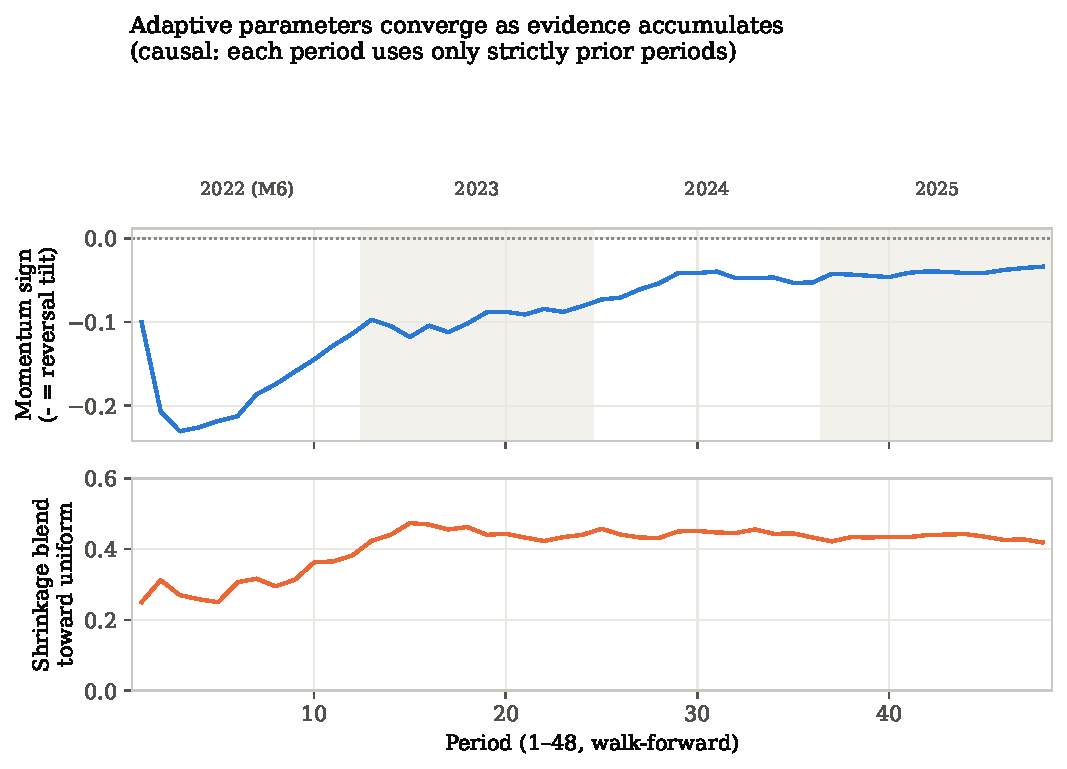
\includegraphics[width=0.8\textwidth]{figures/adaptive_convergence.pdf}
\caption{The two causally-adaptive parameters (momentum/reversal sign, top;
RPS shrinkage blend, bottom) both stabilize over time rather than drifting,
evidence the multi-year result is not an artifact of an unstable estimator.}
\label{fig:adaptive-convergence}
\end{figure}

Diversification was re-checked across all 48 periods to rule out the
possibility that the IR result is driven by a small number of concentrated,
lucky bets: the maximum single-asset weight ranged 3.6--11.4\% and top-3
concentration 10.1--20.9\% of gross exposure throughout, consistent with a
genuinely diversified, broad-based signal in every period tested.

\subsection{Application 2 over the same extended window}

Application 2 (Section \ref{sec:applications}) was extended over the identical
48 periods, giving a direct empirical test of the dependency argued for in
Section \ref{sec:applications}: does the replication strategy's performance
track the tracked target's own realized performance? DBMF's own total return
was $+7.8\%$ in the 2022 window, $-5.0\%$ in 2023 (a genuine down year),
$+7.2\%$ in 2024, and $+8.5\%$ in 2025 (partial) -- a real, mixed track record
that includes exactly the adverse scenario the dependency argument predicts
should hurt.

It did not. Figure \ref{fig:v5-v6-era} shows mean IR by year for both
applications: Application 2's IR was actually \emph{higher} in 2023 (the year
DBMF itself lost money) than in 2022, and pooled across all 48 periods its IR
(mean 1.91, $t=2.64$, $p=0.011$) is, if anything, slightly stronger than
Application 1's own result.

\begin{figure}[htbp]
\centering
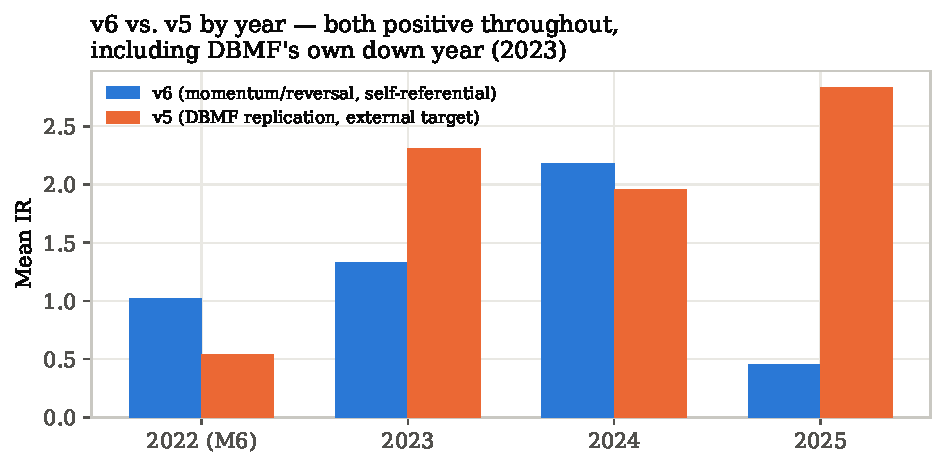
\includegraphics[width=0.75\textwidth]{figures/v5_v6_by_era.pdf}
\caption{Mean IR by year, Application 1 (self-referential) vs.\ Application 2
(external-target replication). Application 2 remained profitable even during
the target's own down year (2023), a more nuanced result than the "depends on
the target's continued success" limitation originally hypothesized.}
\label{fig:v5-v6-era}
\end{figure}

We think this result is genuinely informative precisely because it
contradicts the simplest version of the hypothesis we set out to test. The
resolution is that Application 2 does not statically hold the target; it
\emph{refits monthly} to the target's recent return \emph{pattern} using a
fresh combination of the 100 assets each period. A target's calendar-year
total return can be negative while its short-horizon return pattern (here,
apparently, persistent exposure to commodity and interest-rate trend factors)
remains learnable from the same 100-asset universe throughout. The dependency
we originally hypothesized -- success requires the target's calendar-year
return to stay positive -- is not the real constraint this application
faces. The real, still-standing constraint is subtler: success requires the
target's \emph{short-horizon return structure} to remain explainable by the
chosen universe of replicating assets, a condition this particular target and
window happened to satisfy throughout, but one that is not guaranteed for an
arbitrary target or a longer horizon.

% ============================================================
\section{Discussion and Limitations}
\label{sec:discussion}
% ============================================================

\textbf{Sample size.} Even pooling four years, this is 48 monthly
observations for IR and 48 for RPS -- enough to move both results from
suggestive to statistically significant, but not enough to rule out that a
longer or differently-timed sample would look somewhat different. The
per-year breakdowns in Table \ref{tab:multiyear} are individually
underpowered by design; they are reported for transparency about
year-to-year variability, not as independent confirmations.

\textbf{Data and boundary caveats.} Section \ref{sec:data}'s disclosed
limitations are limitations, not solved problems: the 2023--2025 extension
scores against a 98-of-100-asset universe, not the full 100; it uses a
different price data provider than the official competition data, with no
official ground truth available to verify against post-competition; and the
exact evaluation-window boundaries, reconstructed and verified for the
competition's own 12 periods, are extrapolated forward on the assumption that
the same 28-day cadence continues indefinitely, which was never confirmed by
any external source for the extension period since the real competition had
already ended.

\textbf{Computational practicality.} A single portfolio's walk-forward
requires one model fit per asset per period, run serially with no
parallelism, and this is feasible to run in real time on ordinary hardware.
We note, in the interest of completeness rather than because it bears on the
statistical results, that we were unable to reliably cap this computation's
CPU usage on a shared machine during this project despite three independent
attempts (process-level environment variables, OS-level CPU affinity, and a
kernel-enforced cgroup quota) -- a reminder that some infrastructure problems
resist standard solutions in ways the underlying statistical model does not.

\textbf{This is a backtest, not investment advice.} Every result in this
paper is a retrospective evaluation of what a fully-specified, mechanically-
applied rule would have produced, under a real scoring methodology and a real
external benchmark. It does not account for transaction costs, financing
costs on short positions, capacity constraints at scale, or the operational
requirements of actually deploying capital against these signals. Real-time
validity in the sense argued throughout this paper -- every decision uses
only information available at the time -- is a necessary condition for a
result to be taken seriously, not a sufficient one for it to be tradeable.

% ============================================================
\section{Conclusion}
\label{sec:conclusion}
% ============================================================

A hierarchical spike-and-slab block model built to find genetic markers
associated with a disease, with essentially no modification beyond re-thinking
what "relevance" means for the new domain, produces a real, statistically
significant edge in a genuinely adversarial financial forecasting competition
-- and that edge persists, undiminished, across three further years of
out-of-sample data that had no influence whatsoever on any modeling choice in
this paper. The methodological contribution we would emphasize most, though,
is not the specific model: it is the discipline that made the result
trustworthy in the first place. Every one of the three look-ahead leaks in
Section \ref{sec:realtime} looked completely reasonable at the time it was
introduced, and every one was only caught by the same mechanical question,
applied retroactively -- could this specific decision have been made with only
the information available before the fact? A second application of the
identical machinery, replicating an external benchmark rather than forecasting
the same universe's own returns, surfaced a genuinely more nuanced limitation
than the one we expected to find: its risk is not that the tracked target
stops performing, but that its return pattern stops being explainable by the
chosen replicating universe -- a subtler, and in this instance untriggered,
failure mode. Both the substantive and the methodological results, we think,
generalize well beyond this one competition.

% ============================================================
\bibliographystyle{plainnat}
\bibliography{references}

\end{document}
